\documentclass[a4paper]{article}
\usepackage[affil-it]{authblk}
\usepackage[english]{babel}
\usepackage[backend=bibtex,style=numeric]{biblatex}

\usepackage{geometry}
\geometry{margin=1.5cm, vmargin={0pt,1cm}}
\setlength{\topmargin}{-1cm}
\setlength{\paperheight}{29.7cm}
\setlength{\textheight}{25.3cm}

% useful packages.
\usepackage{amsfonts}
\usepackage{amsmath}
\usepackage{amssymb}
\usepackage{amsthm}     
\usepackage{enumerate} %enumerate environment
\usepackage{graphicx}
\usepackage{multicol}
\usepackage{fancyhdr}
\usepackage{layout}
\usepackage{ctex}      %中文环境
\usepackage{booktabs}  %三线表
\usepackage{verbatim}  %comment environment
\usepackage{float}     %强制表格图片位置
\usepackage{listings}  %insert code in latex
\usepackage{fontspec}  %font support
\usepackage{tikz}
\usepackage{makecell}
\usetikzlibrary{intersections}
\usepackage{arydshln}

\usepackage[colorlinks,linkcolor=blue]{hyperref}
\usepackage{xcolor}
\definecolor{mygreen}{rgb}{0,0.6,0}
\definecolor{lightgrey}{rgb}{0.95,0.95,0.95}
\definecolor{winered}{rgb}{0.5,0,0}
\definecolor{mymauve}{rgb}{0.58,0,0.82}
\lstset{
      backgroundcolor=\color{lightgrey},
      basicstyle             = \ttfamily,
      breakatwhitespace      = false,
      breaklines             = true,
      captionpos             = none,
      commentstyle           = \color{mygreen}\bfseries,
      extendedchars          = false,
      keepspaces             = true,
      keywordstyle           = \color{winered},         % keyword style
      language               = C++,                     % the language of code
      otherkeywords          = {string},
      numberstyle            = \tiny\color{mygray},
      rulecolor              = \color{black},
      showspaces             = false,
      showstringspaces       = false,
      showtabs               = false,
      stepnumber             = 1,
      stringstyle            = \color{mymauve},         % string literal style
      tabsize                = 2,
      title                  = \lstname,
      aboveskip              = 0pt,
      belowskip              = 0pt,
      columns                = flexible
}

% some common command
\newcommand{\dif}{\mathrm{d}}
\newcommand{\avg}[1]{\left\langle #1 \right\rangle}
\newcommand{\norm}[1]{\left\| #1 \right\|}
\newcommand{\difFrac}[2]{\frac{\dif #1}{\dif #2}}
\newcommand{\pdfFrac}[2]{\frac{\partial #1}{\partial #2}}
\newcommand{\OFL}{\mathrm{OFL}}
\newcommand{\UFL}{\mathrm{UFL}}
\newcommand{\fl}{\mathrm{fl}}
\newcommand{\op}{\odot}
\newcommand{\Eabs}{E_{\mathrm{abs}}}
\newcommand{\Erel}{E_{\mathrm{rel}}}
\addbibresource{citation.bib}

\begin{document}
% =================================================
\title{Numerical Analysis chapter 3 theoretical homework}

\author{Zhouyue Qian 3220104074
  \thanks{Electronic address: \texttt{3220104074@edu.zju.cn}}}
\affil{(Information and Computational Science Class 2201), Zhejiang University }


\date{Due time: \today}

\maketitle

%\begin{abstract}
%    The abstract is not necessary for the theoretical homework, 
%    but for the programming project, 
%    you are encouraged to write one.      
%\end{abstract}





% ============================================
\section*{I}
\textbf{Proof:}

\[p(1) =1, p^{'}(1)=-3,p^{''}(1)=6,s(0) =0\]
We assume that $p(x) = a_0 + a_1x + a_2x^2 + a_3x^3$.
We have: $a_0 = 0, a_1=12, a_2=-18, a_3=7$
$p^{''}(0)=-36\neq 0$
So $s(x)$ is not a natural cubic spline.

\section*{II}
\subsection*{a}
If we want to determine $s$ uniquely, we need to have $3*(n-1)=3n-3$ conditions.
From $s_i = f_i$, we have $n$ conditions.
From $s^{'}_i = s^{'}_{i+1}$, we have $n-2$ conditions.
From $s^{''}_i = s^{''}_{i+1}$, we have $n-2$ conditions.
We have $3n-4$ conditions in total, so $s$ can not be uniquely determined.

\subsection*{b}
$m_i = s^{'}(x_i), p_i = s|_{[x_i,x_{i+1}]},p_i(x_i)=f(x_i),p_i(x_{i+1})=f(x_{i+1})$
\begin{align*}
    p_i(x) &= f_i + m_i(x-x_i) + \frac{f[x_i,x_{i+1}]-m_i}{x_{i+1}-x_i}(x-x_i)^2 \\
           &= f_i + m_i(x-x_i) + \frac{\frac{f_{i+1}-f_i}{x_{i+1}-x_i}-m_i}{x_{i+1}-x_i}(x-x_i)^2\\
           &= f_i + m_i(x-x_i) + \frac{f_{i+1}-f_i-m_i(x_{i+1}-x_i)}{(x_{i+1}-x_i)^2}(x-x_i)^2
\end{align*}

\subsection*{c}
$$p^{'}_i = m_i + 2(x - x_i)\frac{f_{i+1}-f_i-m_i(x_{i+1}-x_i)}{(x_{i+1}-x_i)^2}$$
$$p^{'}_{i+1} = m_{i+1}+2(x - x_{i+1})\frac{f_{i+2}-f_{i+1}-m_{i+1}(x_{i+2}-x_{i+1})}{(x_{i+2}-x_{i+1})^2}$$
$$p^{'}_i(x_{i+1})=p^{'}_{i+1}(x_{i+1})$$
$$m_{i+1}= m_i + 2\frac{f_{i+1}-f_i-m_i(x_{i+1}-x_i)}{(x_{i+1}-x_i)}$$

\section*{III}
\[
\left\{
\begin{aligned}
s_1(x) &= 1 + c(x+1)^3, \\
s_1'(x) &= 3c(x+1)^2, \\
s_2''(x) &= 6c(x+1),
\end{aligned}
\right.
\left\{
\begin{aligned}
s_2(0) &= 1 + c, \\
s_2'(0) &= 3c, \\
s_2''(0) &= 6c, \\
s_2(1) &= 0.
\end{aligned}
\right.
\]
We have $s_2(x) = 1 + c + 3cx + 3cx^2 - cx^3$ and $s_2(1) = -1$, so $c = -\frac{1}{3}$.

\section*{IV}
$f(x) = cos(\frac{\pi }{2}x),x\in [-1,1]$
\subsection*{a}
\[
\left\{
\begin{aligned}
  f(x) = cos(\frac{\pi }{2}x)\\
  f'(x) = -\frac{\pi}{2}sin(\frac{\pi }{2}x)\\
  f''(x) = -\frac{\pi^2}{4}cos(\frac{\pi }{2}x)
\end{aligned}
\right.
\]
We have $M_1 = s''(-1) = 0, s''(1)=0=M_3$ and we know $f(-1)=0,f(1)=0,f(0) = 1$
From \textbf{lemma 3.4}, we have $$\mu_2M_1+2M_2+\lambda_2M_3 = 6f[-1,0,1].$$
It is trivial that $f[-1,0,1]=-1,\mu_2 = \frac{1}{2},\lambda_2 = \frac{1}{2}$.So, we have $M_2 = -3$.
\[
\left\{
\begin{aligned}
  s''(0) = -3\\
  s''(1) = 0\\
  s''(-1) = 0.
\end{aligned}
\right.
\]
We have 
\[s(x) = 
\begin{cases} 
-\frac{1}{2}x^3 - \frac{3}{2}x^2 + 1, & \text{if } x \in [-1,0] \\
\frac{1}{2}x^3 - \frac{3}{2}x^2 + 1, & \text{if } x \in [0,1]
\end{cases}\]

\subsection*{b}
$g(-1)=0,g(0)=1,g(1)=0$
\subsubsection*{i}
It is obvious that $g(x)= -x^2+1$.
$$\int_{-1}^{1}[s''(x)]^2dx = \int_{-1}^{0}(-3x-3)^2dx + \int_{0}^{1}(3x-3)^2dx =6$$
$$\int_{-1}^{1}[g''(x)]^2dx  = 8 > \int_{-1}^{1}[s''(x)]^2dx $$
\subsubsection*{ii}
$$\int_{-1}^{1}[f''(x)]^2dx = \frac{\pi^4}{16}>6$$

\section*{V}
\subsection*{a}
\[
B^0_i=
\begin{cases}
1, & \text{if } x \in [t_{i-1},t_{i}] \\
0, & \text{otherwise}
\end{cases}
\]
\[
  \hat{B_i}(x)=
  \begin{cases}
  \frac{x-t_{i-1}}{t_{i}-t_{i-1}}, x \in [t_{i-1},t_{i}] \\
  \frac{t_{i+1}-x}{t_{i+1}-t_{i}}, x \in [t_{i},t_{i+1}] \\
  0, \text{otherwise}
  \end{cases}
\]
\[
  B^{n+1}_{i}=\frac{x-t_{i-1}}{t_{i+n}-t_{i-1}}B^n_i(x)+\frac{t_{i+n+1}-x}{t_{i+n+1}-t_i}B^n_{i+1}(x)
\]
\[
B^2_i(x) =
\begin{cases} 
\frac{(x - t_{i-1})^2}{(t_{i+1} - t_{i-1})(t_i - t_{i-1})}, & x \in (t_{i-1}, t_i] \\[12pt]
\frac{(x - t_{i-1})(t_{i+1} - x)}{(t_{i+1} - t_{i-1})(t_{i+1} - t_i)} + \frac{(t_{i+2} - x)(x - t_i)}{(t_{i+2} - t_i)(t_{i+1} - t_i)}, & x \in (t_i, t_{i+1}] \\[12pt]
\frac{(t_{i+2} - x)^2}{(t_{i+2} - t_i)(t_{i+2} - t_{i+1})}, & x \in (t_{i+1}, t_{i+2}] \\[12pt]
0, & \text{otherwise}.
\end{cases}
\]
\subsection*{b}
\[
\frac{d}{dx}B^2_i(x) =
\begin{cases}
\frac{2(x - t_{i-1})}{(t_{i+1} - t_{i-1})(t_i - t_{i-1})}, & x \in (t_{i-1}, t_i] \\
\frac{t_{i+1} - 2x + t_{i+1}}{(t_{i+1} - t_{i-1})(t_{i+1} - t_i)} + \frac{t_{i+2} - 2x + t_i}{(t_{i+2} - t_i)(t_{i+1} - t_i)}, & x \in (t_i, t_{i+1}] \\
\frac{-2(t_{i+2} - x)}{(t_{i+2} - t_i)(t_{i+2} - t_{i+1})}, & x \in (t_{i+1}, t_{i+2}] \\
0, & \text{otherwise}.
\end{cases}
\]
We have $$\lim_{x \to t_i^+}(\frac{t_{i+1} - 2x + t_{i+1}}{(t_{i+1} - t_{i-1})(t_{i+1} - t_i)} + \frac{t_{i+2} - 2x + t_i}{(t_{i+2} - t_i)(t_{i+1} - t_i)})=\frac{2}{t_{i+1}-t_{i-1}} $$
$$\lim_{x \to t_{i+1}^+}(\frac{-2(t_{i+2} - x)}{(t_{i+2} - t_i)(t_{i+2} - t_{i+1})}) = \frac{-2}{t_{i+2}-t_i}$$
So $B^2_i(x)$ is $C^1$ continuous.

\subsection*{c}
From the deritive of $B^2_i(x)$, we have $B^2_i(x)$ increase from $t_{i-1}$ to $t_i$ and decrease from $t_i$ to $t_{i+1}$.
We have $B^2_i(t_i)> 0$ and $B^2_i(t_{i+1}) < 0$ in $[t_{i-1},t_{i+1}]$.
From the continuity of $\frac{d}{dx}B^2_i(x)$, we have $B^2_i(x)$ has a zero point in $[t_{i-1},t_{i+1}]$.

\subsection*{d}
We assume that the zero point of $\frac{d}{dx}B^2_i(x)$ is $x^*$.
\[
\frac{d}{dx}B^2_i(x) =
\begin{cases}
  >0, & x \in (t_{i-1}, x^*) \\
  =0, & x = x^* \\
  <0, & x \in (x^*, t_{i+2})\\
  0, & \text{otherwise}
\end{cases}
\]
So $\max B^2_i(x^*)= \frac{t_{i+2}-t_{i-1}}{t_{i+2}-t_{i-1}+t_{i+1}-t_i}<1$ and $\min B^2_i(x^*)=0$.
So $B^2_i(x) \in [0,1)$

\subsection*{e}
Let $t_i = i$ we have
\[
B^2_i(x) =
\begin{cases}
\frac{(x - i + 1)^2}{2}, & x \in (i-1, i] \\
\frac{(x - i + 1)(- x + i + 1) + (x - i)(-x + i + 2)}{2}, & x \in (i, i+1] \\
\frac{(-x + i + 2)^2}{2}, & x \in (i+1, i+2] \\
0, & \text{otherwise}.
\end{cases}
\]

\begin{figure}[H]
  \centering
  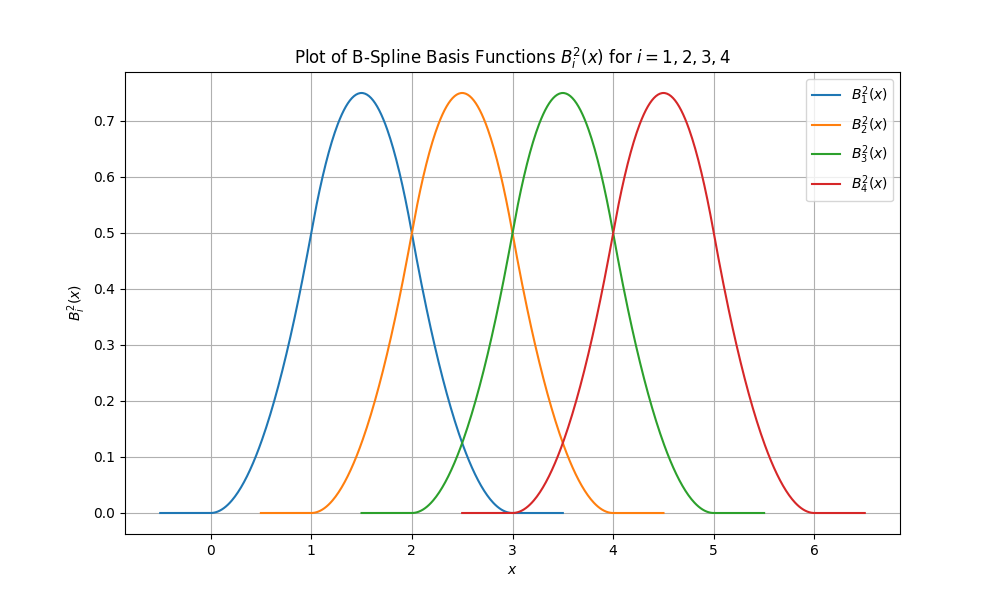
\includegraphics[width=0.8\textwidth]{e.png}
  \caption{The graph of $B^2_i(x)$}
\end{figure}

\section*{VI}
$$B^n_i(x)=(t_{i+n}-t_{i-1})[t_{i-1},\cdots t_{i+n}](t-x)_{+}^{n},\forall n$$
When $n = 2$, $B^2_i(x)=(t_{i+2}-t_{i-1})[t_{i-1}\cdots t_{i+2}](t-x)_{+}^{2}.$
$$B^{n+1}_{i}=\frac{x-t_{i-1}}{t_{i+n}-t_{i-1}}B^n_i(x)+\frac{t_{i+n+1}-x}{t_{i+n+1}-t_i}B^n_{i+1}(x)$$
$$B^0_i(x) = (t_i - t_{i-1})[t_{i-1},t_i](t-x)^0_+$$
$$\therefore B^1_i(x) = (x - t_{i-1})[t_{i-1},t_i](t-x)_{+}^{0}+(t_{i+1}-x)[t_i,t_{i+1}](t-x)_+^0$$
$$(t_{i-1}\cdots t_{i+n})()_+^{n+1} = (t_{i-1}-x)[t_{i-1}\cdots t_{i+n}](t-x)_{+}^n$$
$$ \implies B^1_i(x) = (t_{i+1}-t_{i-1})[t_{i-1},t_i,t_{i+1}](t-x)_+^n$$
Similarly, we have
  \begin{align*}
    B^2_i(x) &= (x - t_{i-1})[t_{i-1}, t_i, t_{i+1}](t - x)_+^1 + (t_{i+2} - x)[t_i, t_{i+1}, t_{i+2}](t - x)_+^1 \\
    &= -[t_{i-1}, t_i, t_{i+1}](t - x)_+^2 + [t_i, t_{i+1}, t_{i+2}](t - x)_+^2 \\
    &= (t_{i+2} - t_{i-1})[t_{i-1}, t_i, t_{i+1}, t_{i+2}](t - x)_+^2
  \end{align*}

The proof is completed.

\section*{VII}
\[
  \frac{d}{dx}B_i^n(x) = n(\frac{B_i^{n-1}(x)}{t_{i+n-1}-t_{i-1}}-\frac{B_{i+1}^{n-1}(x)}{t_{i+n}-t_{i}})
\]
\[
  \int_{t_{i-1}}^{t_{i+n}}\frac{d}{dx}B_i^n(x)dx = 0
\]
This is because the derivative of $B_i^n(x)$ is continuous and $B^n_i(t_{i-1})=B^n_i(t_{i+n})=0$
\[
  \therefore \int_{t_{t+n+1}}^{t_{i-1}} \frac{d}{dx}B_i^n(x) \,dx \\
  \implies \int_{t_{i-1}}^{i+n} \frac{B^{n-1}_i(x)}{t_{i+n-1}-t_{i-1}} \,dx = \int_{t_i}^{t_{i+n}} \frac{B^{n-1}_{i+1}(x)}{t_{i+n}-t_i} \,dx \Box  
\]

\section*{VIII}
$$\tau_{m-n}(x_i \cdots x_{i+n}) = [x_i,x_{i+1}\cdots x_{i+n}]x^m$$
\subsection*{a}
$$\tau_{2}(x_i \cdots x_{i+2}) = [x_i,x_{i+1},x_{i+2}]x^4$$ 
\[
  \begin{array}{c|ccc}
  x_i & x_i^4 & &  \\
  x_{i+1} & x_{i+1}^4 & (x_{i+1}^3+x_{i}x_{i+1}^2+x_i^2x_{i+1}+x_i^3) &  \\
  x_{i+2} & x_{i+2}^4 & (x_{i+2}^3+x_{i+1}x_{i+2}^2+x_{i+1}^2x_{i+2}+x_{i+1}^3) &x_i^2+x_{i+1}^2+x_{i+2}^2+x_{i+1}x_{i+2}+x_ix_{i+1}+x_ix_{i+2}  
  \end{array}
\]
The proof is completed.

\subsection*{b}
\begin{align*}
  (x_{n+1}-x_1)\tau_k(x_1 \cdots x_{n+1}) &= \tau_{k+1}(x_1\cdots x_{n+1})-\tau_{k+1}(x_1\cdots x_{n})-x_1\tau_k(x_1\cdots x_{n+1}) \\
  &=\tau_{k+1}(x_2\cdots x_{n+1})-\tau_{k+1}(x_1 \cdot x_n) \\
\end{align*}
$n = 0 : \tau_m(x_i)=[x_i]x^m$

$k = n+1:$\\
\begin{align*}
  \tau_{m-n-1}(x_i\cdots x_{i+n+1}) &= \frac{\tau_{m-n}(x_{i+1}\cdots x_{i+n+1})-\tau_{m-n}(x_i\cdots x_{i+n})}{x_{i+n+1}-x_i} \\
  &= \frac{[x_{i+1},x_{i+2}\cdots x_{i+n+1}]x^{m}-[x_i\cdots x_{i+n}]x^m}{x_{i+n+1}-x_i} \\
  &= [x_i,x_{i+1}\cdots x_{i+n+1}]x^{m}
\end{align*}
The proof is completed.\cite*{openai2024chatgpt}
\section*{ \center{\normalsize {Acknowledgement}} }
\printbibliography


\end{document}